%\documentclass[onecolumn]{article}
%\usepackage{amsmath}
%\usepackage{enumerate}
%\usepackage{enumitem}
%\usepackage{listings}
%\usepackage[utf8]{inputenc}
%\usepackage{amssymb}
%\usepackage{tabularx}
%\usepackage{tikz}
%\usetikzlibrary{arrows,positioning,shapes.geometric}
%\usepackage{booktabs}
%\usepackage{multirow}
%\usepackage{siunitx}
%\usepackage{graphicx}
%\def\inputGnumericTable{}
%\usepackage{fullpage}
%\usepackage{color}
%\usepackage{array}
%\usepackage{longtable}
%\usepackage{calc}
%\usepackage{multirow}
%\usepackage{hhline}
%\usepackage{ifthen}
%\graphicspath{{./images/}}
%\usepackage[big]{titlesec}
%\usepackage{titlesec}

%%\titleformat*{\section}{\huge\bfseries}
%\titleformat*{\subsection}{\huge\bfseries}
%\titleformat*{\subsubsection}{\huge\bfseries}
%\lstset{
  %  frame=single,
  %  breaklines=true
%}
%\usepackage{hyperref}
%\usepackage[a3paper,outer=1.5cm,inner=1.5cm,top=1.75cm,bottom=1.5cm]{geometry}
%\def\mytitle{\textbf{DEMODULATION TECHNIQUES}}
%\def\myauthor{DUDEKULA USENI}
%\def\contact{r171099@rguktrkv.ac.in}

%\def\contact{r171099@rguktrkv.ac.in }
%\def\mymodule{Future Wireless Communication (FWC)}

%\thiswatermark{\centering \put(-15,-100.0){\includegraphics[scale=0.4]{iith.png}} }
%\title{\mytitle}
%\author{\myauthor\hspace{1em}\\\contact\ FWC22098 -\hspace{0.5em}IITH \hspace{0.5em}\mymodule\hspace{6em}}

%\providecommand{\mbf}{\mathbf}
%\newcommand{\myvec}[1]{\ensuremath{\begin{pmatrix}#1\end{pmatrix}}}
%\providecommand{\qfunc}[1]{\ensuremath{Q\left(#1\right)}}
%\providecommand{\cbrak}[1]{\ensuremath{\left\{#1\right\}}}
%\providecommand{\brak}[1]{\ensuremath{\left(#1\right)}}
%\providecommand{\lsbrak}[1]{\ensuremath{{}\left[#1\right.}}
%\providecommand{\rsbrak}[1]{\ensuremath{{}\left.#1\right]}}
%\providecommand{\rcbrak}[1]{\ensuremath{\left.#1\right\}}}
%\providecommand{\lcbrak}[1]{\ensuremath{\left\{#1\right.}}
%\providecommand{\sbrak}[1]{\ensuremath{{}\left[#1\right]}}

%\begin{document}
%%\begin{enumerate}
%\begin{Large}


\section{what is Demodulation}
%\item[\textbf{}] 

Demodulation is the process of extracting the original information or baseband signal from a modulated carrier signal.The purpose of demodulation is to retrieve the modulating signal, which could be analog or digital data, audio, video, or other forms of information. Demodulation is essential in various communication systems such as radio, television, cellular networks, and wireless data transmission.
%\end{Large}\\


The demodulation code used in NavIC may vary depending on the specific implementation and receiver hardware. However, I can provide you with a general outline of the demodulation process for NavIC signals.

NavIC signals are transmitted in the L5 frequency band (1176.45 MHz) using BPSK modulation for the navigation message and various modulation schemes (such as BOC and MBOC) for the ranging signal. The demodulation process typically involves the following steps:

\textbf{Signal Acquisition:} The receiver searches for and acquires the NavIC signal by correlating the received signal with a locally generated replica of the spreading code used by the satellites. This process helps in identifying the presence of the NavIC signal and estimating the initial timing offset.

\textbf{Carrier Tracking:} Once the signal is acquired, the receiver performs carrier tracking to estimate and track the carrier frequency and phase of the received signal. This is crucial for demodulation as it ensures accurate demodulation of the navigation message and ranging signal.

\textbf{Code Tracking:} The receiver performs code tracking to estimate and track the spreading code used by the satellites. This helps in maintaining synchronization with the transmitted signal and extracting the navigation data and ranging information.

\textbf{Data Extraction:} Once the demodulation is performed, the receiver extracts the navigation data from the demodulated signal. The navigation data includes information such as satellite ephemeris, clock correction, and other parameters necessary for calculating the receiver's position, velocity, and timing.

\subsection{Signal Acquistion}
\begin{normalsize}
\begin{figure}[!h]%
\centering%
%\rule{30pt}{20pt}%
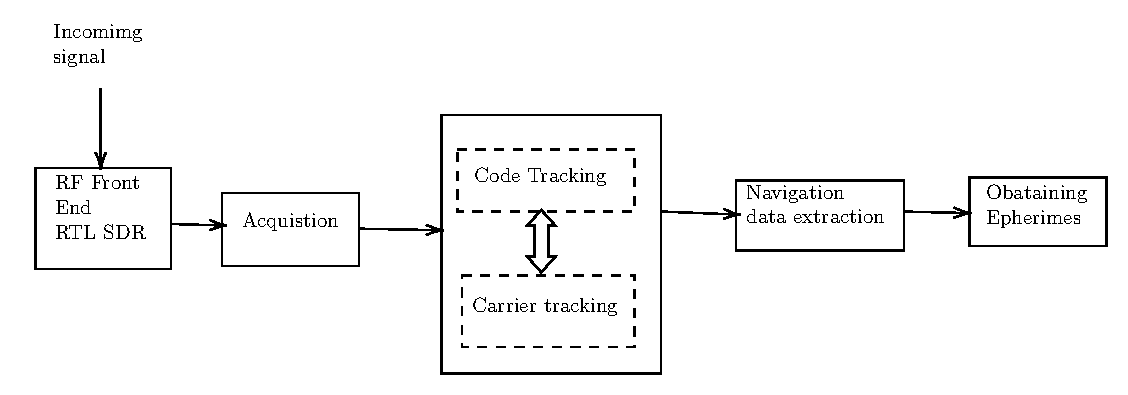
\includegraphics[scale=0.5]{figs/block2}
\end{figure} 

\end{normalsize}
\begin{center}
Figure2 : The Block Level Architecture in Demodulation
\end{center}
A generic IRNSS signal defined by its complex baseband equivalent, 
$S_T(t)$, the digital signal at the input of an Acquisition block can be written as:
\begin{align}
x_{IN}[k]=A(t)\hat S_T (t-\tau(t))e^{j(2 \pi f_D(t)t+\Phi))}\bigg|_{t=kT_s} +n(t)\bigg|_{t=kT_s}
\end{align}
%\end{Large}
\begin{table}[h]
\centering
	\caption{\Large{Parameters Table in Signal Acquisition}}
	%%%%%%%%%%%%%%%%%%%%%%%%%%%%%%%%%%%%%%%%%%%%%%%%%%%%%%%%%%%%%%%%%%%%%%
%%                                                                  %%
%%  This is the header of a LaTeX2e file exported from Gnumeric.    %%
%%                                                                  %%
%%  This file can be compiled as it stands or included in another   %%
%%  LaTeX document. The table is based on the longtable package so  %%
%%  the longtable options (headers, footers...) can be set in the   %%
%%  preamble section below (see PRAMBLE).                           %%
%%                                                                  %%
%%  To include the file in another, the following two lines must be %%
%%  in the including file:                                          %%
%%        \def\inputGnumericTable{}                                 %%
%%  at the beginning of the file and:                               %%
%%        \input{name-of-this-file.tex}                             %%
%%  where the table is to be placed. Note also that the including   %%
%%  file must use the following packages for the table to be        %%
%%  rendered correctly:                                             %%
%%    \usepackage[latin1]{inputenc}                                 %%
%%    \usepackage{color}                                            %%
%%    \usepackage{array}                                            %%
%%    \usepackage{longtable}                                        %%
%%    \usepackage{calc}                                             %%
%%    \usepackage{multirow}                                         %%
%%    \usepackage{hhline}                                           %%
%%    \usepackage{ifthen}                                           %%
%%  optionally (for landscape tables embedded in another document): %%
%%    \usepackage{lscape}                                           %%
%%                                                                  %%
%%%%%%%%%%%%%%%%%%%%%%%%%%%%%%%%%%%%%%%%%%%%%%%%%%%%%%%%%%%%%%%%%%%%%%



%%  This section checks if we are begin input into another file or  %%
%%  the file will be compiled alone. First use a macro taken from   %%
%%  the TeXbook ex 7.7 (suggestion of Han-Wen Nienhuys).            %%
\def\ifundefined#1{\expandafter\ifx\csname#1\endcsname\relax}


%%  Check for the \def token for inputed files. If it is not        %%
%%  defined, the file will be processed as a standalone and the     %%
%%  preamble will be used.                                          %%
\ifundefined{inputGnumericTable}

%%  We must be able to close or not the document at the end.        %%
	\def\gnumericTableEnd{\end{document}}


%%%%%%%%%%%%%%%%%%%%%%%%%%%%%%%%%%%%%%%%%%%%%%%%%%%%%%%%%%%%%%%%%%%%%%
%%                                                                  %%
%%  This is the PREAMBLE. Change these values to get the right      %%
%%  paper size and other niceties.                                  %%
%%                                                                  %%
%%%%%%%%%%%%%%%%%%%%%%%%%%%%%%%%%%%%%%%%%%%%%%%%%%%%%%%%%%%%%%%%%%%%%%

	\documentclass[12pt%
			  %,landscape%
                    ]{report}
       \usepackage[latin1]{inputenc}
       \usepackage{fullpage}
       \usepackage{color}
       \usepackage{array}
       \usepackage{longtable}
       \usepackage{calc}
       \usepackage{multirow}
       \usepackage{hhline}
       \usepackage{ifthen}

	\begin{document}


%%  End of the preamble for the standalone. The next section is for %%
%%  documents which are included into other LaTeX2e files.          %%
\else

%%  We are not a stand alone document. For a regular table, we will %%
%%  have no preamble and only define the closing to mean nothing.   %%
    \def\gnumericTableEnd{}

%%  If we want landscape mode in an embedded document, comment out  %%
%%  the line above and uncomment the two below. The table will      %%
%%  begin on a new page and run in landscape mode.                  %%
%       \def\gnumericTableEnd{\end{landscape}}
%       \begin{landscape}


%%  End of the else clause for this file being \input.              %%
\fi

%%%%%%%%%%%%%%%%%%%%%%%%%%%%%%%%%%%%%%%%%%%%%%%%%%%%%%%%%%%%%%%%%%%%%%
%%                                                                  %%
%%  The rest is the gnumeric table, except for the closing          %%
%%  statement. Changes below will alter the table's appearance.     %%
%%                                                                  %%
%%%%%%%%%%%%%%%%%%%%%%%%%%%%%%%%%%%%%%%%%%%%%%%%%%%%%%%%%%%%%%%%%%%%%%

\providecommand{\gnumericmathit}[1]{#1} 
%%  Uncomment the next line if you would like your numbers to be in %%
%%  italics if they are italizised in the gnumeric table.           %%
%\renewcommand{\gnumericmathit}[1]{\mathit{#1}}
\providecommand{\gnumericPB}[1]%
{\let\gnumericTemp=\\#1\let\\=\gnumericTemp\hspace{0pt}}
 \ifundefined{gnumericTableWidthDefined}
        \newlength{\gnumericTableWidth}
        \newlength{\gnumericTableWidthComplete}
        \newlength{\gnumericMultiRowLength}
        \global\def\gnumericTableWidthDefined{}
 \fi
%% The following setting protects this code from babel shorthands.  %%
 \ifthenelse{\isundefined{\languageshorthands}}{}{\languageshorthands{english}}
%%  The default table format retains the relative column widths of  %%
%%  gnumeric. They can easily be changed to c, r or l. In that case %%
%%  you may want to comment out the next line and uncomment the one %%
%%  thereafter                                                      %%
\providecommand\gnumbox{\makebox[0pt]}
%%\providecommand\gnumbox[1][]{\makebox}

%% to adjust positions in multirow situations                       %%
\setlength{\bigstrutjot}{\jot}
\setlength{\extrarowheight}{\doublerulesep}

%%  The \setlongtables command keeps column widths the same across  %%
%%  pages. Simply comment out next line for varying column widths.  %%
\setlongtables

\setlength\gnumericTableWidth{%
	68pt+%
	235pt+%
0pt}
\def\gumericNumCols{2}
\setlength\gnumericTableWidthComplete{\gnumericTableWidth+%
         \tabcolsep*\gumericNumCols*2+\arrayrulewidth*\gumericNumCols}
\ifthenelse{\lengthtest{\gnumericTableWidthComplete > \linewidth}}%
         {\def\gnumericScale{\ratio{\linewidth-%
                        \tabcolsep*\gumericNumCols*2-%
                        \arrayrulewidth*\gumericNumCols}%
{\gnumericTableWidth}}}%
{\def\gnumericScale{1}}

%%%%%%%%%%%%%%%%%%%%%%%%%%%%%%%%%%%%%%%%%%%%%%%%%%%%%%%%%%%%%%%%%%%%%%
%%                                                                  %%
%% The following are the widths of the various columns. We are      %%
%% defining them here because then they are easier to change.       %%
%% Depending on the cell formats we may use them more than once.    %%
%%                                                                  %%
%%%%%%%%%%%%%%%%%%%%%%%%%%%%%%%%%%%%%%%%%%%%%%%%%%%%%%%%%%%%%%%%%%%%%%

\ifthenelse{\isundefined{\gnumericColA}}{\newlength{\gnumericColA}}{}\settowidth{\gnumericColA}{\begin{tabular}{@{}p{68pt*\gnumericScale}@{}}x\end{tabular}}
\ifthenelse{\isundefined{\gnumericColB}}{\newlength{\gnumericColB}}{}\settowidth{\gnumericColB}{\begin{tabular}{@{}p{235pt*\gnumericScale}@{}}x\end{tabular}}

\begin{longtable}[c]{%
	b{\gnumericColA}%
	b{\gnumericColB}%
	}

%%%%%%%%%%%%%%%%%%%%%%%%%%%%%%%%%%%%%%%%%%%%%%%%%%%%%%%%%%%%%%%%%%%%%%
%%  The longtable options. (Caption, headers... see Goosens, p.124) %%
%	\caption{The Table Caption.}             \\	%
% \hline	% Across the top of the table.
%%  The rest of these options are table rows which are placed on    %%
%%  the first, last or every page. Use \multicolumn if you want.    %%

%%  Header for the first page.                                      %%
%	\multicolumn{2}{c}{The First Header} \\ \hline 
%	\multicolumn{1}{c}{colTag}	%Column 1
%	&\multicolumn{1}{c}{colTag}	\\ \hline %Last column
%	\endfirsthead

%%  The running header definition.                                  %%
%	\hline
%	\multicolumn{2}{l}{\ldots\small\slshape continued} \\ \hline
%	\multicolumn{1}{c}{colTag}	%Column 1
%	&\multicolumn{1}{c}{colTag}	\\ \hline %Last column
%	\endhead

%%  The running footer definition.                                  %%
%	\hline
%	\multicolumn{2}{r}{\small\slshape continued\ldots} \\
%	\endfoot

%%  The ending footer definition.                                   %%
%	\multicolumn{2}{c}{That's all folks} \\ \hline 
%	\endlastfoot
%%%%%%%%%%%%%%%%%%%%%%%%%%%%%%%%%%%%%%%%%%%%%%%%%%%%%%%%%%%%%%%%%%%%%%

\hhline{|-|-}
	 \multicolumn{1}{|p{\gnumericColA}|}%
	{\gnumericPB{\raggedright}\gnumbox[l]{\hspace{0.75cm}\textbf{Symbol}}}
	&\multicolumn{1}{p{\gnumericColB}|}%
	{\gnumericPB{\raggedright}\gnumbox[l]{\hspace{3cm} \textbf{Definition}}}
\\
\hhline{|--|}
	 \multicolumn{1}{|p{\gnumericColA}|}%
	{\gnumericPB{\raggedright}\gnumbox[l]{\hspace{1cm}$x_{IN}[k]$}}
	&\multicolumn{1}{p{\gnumericColB}|}%
	{\gnumericPB{\raggedright}\gnumbox[l]{complex vector $I,Q$ samples of received signal}}
\\
\hhline{|--|}
	 \multicolumn{1}{|p{\gnumericColA}|}%
	{\gnumericPB{\raggedright}\gnumbox[l]{\hspace{1cm}A(t)}}
	&\multicolumn{1}{p{\gnumericColB}|}%
	{\gnumericPB{\raggedright}\gnumbox[l]{Signal Amplitude}}
\\
\hhline{|--|}
	 \multicolumn{1}{|p{\gnumericColA}|}%
	{\gnumericPB{\raggedright}\gnumbox[l]{\hspace{1cm}$\hat S_T(t)$}}
	&\multicolumn{1}{p{\gnumericColB}|}%
	{\gnumericPB{\raggedright}\gnumbox[l]{filtered version of $S_T(t)$}}
\\
\hhline{|--|}
	 \multicolumn{1}{|p{\gnumericColA}|}%
	{\gnumericPB{\raggedright}\gnumbox[l]{\hspace{1cm}$f_D(t)$ }}
	&\multicolumn{1}{p{\gnumericColB}|}%
	{\gnumericPB{\raggedright}\gnumbox[l]{Time - varing doppler shift}}
\\
\hhline{|--|}
	 \multicolumn{1}{|p{\gnumericColA}|}%
	{\gnumericPB{\raggedright}\gnumbox[l]{\hspace{1cm}$\Phi (t)$}}
	&\multicolumn{1}{p{\gnumericColB}|}%
	{\gnumericPB{\raggedright}\gnumbox[l]{Time - varing carrier phase shift}}
\\
\hhline{|--|}
	 \multicolumn{1}{|p{\gnumericColA}|}%
	{\gnumericPB{\raggedright}\gnumbox[l]{\hspace{1cm}n(t) }}
	&\multicolumn{1}{p{\gnumericColB}|}%
	{\gnumericPB{\raggedright}\gnumbox[l]{Term modelling random noise}}
\\
\hhline{|--|}
	 \multicolumn{1}{|p{\gnumericColA}|}%
	{\gnumericPB{\raggedright}\gnumbox[l]{\hspace{1cm}$T_s$ }}
	&\multicolumn{1}{p{\gnumericColB}|}%
	{\gnumericPB{\raggedright}\gnumbox[l]{sampling period}}
\\
\hhline{|-|-|}
\end{longtable}

\ifthenelse{\isundefined{\languageshorthands}}{}{\languageshorthands{\languagename}}
\gnumericTableEnd

\end{table}
%\begin{Large}



\subsubsection{Implementation of CA PCPS Acquisition}
The Parallel Code Phase Search (PCPS) algorithm is described as follows:
Input signal buffer $x_{IN}$ of k complex samples, acquisition threshold $\gamma$\\
provided by the Signal Conditioner; on-memory FFT of the local replica,
\begin{align}
D[k]=FFT_k\{d[k]\}
\end{align}
\begin{align}
\text{input signal power estimation :} \hat P_{in} = \frac{1}{k}\sum_{k=0}^{k-1} \big| x_{IN}[k]\big| ^2
\end{align}
\begin{align}
\check f_D=[ f_{min}, f_{max}]\hspace{0.5cm} in \hspace{0.5cm}f_{steps} 
\end{align}
\begin{align}
\text{carrier wipe off:}\hspace{0.5cm}x[k]=x_{IN}[k]e^{-(j2 \pi \check f_D k T_s)},\hspace{0.5cm}for\hspace{0.5cm}k=0,...,k-1
\end{align}
\begin{align}
X[k]=FFT_k\{x[k]\}
\end{align}
\begin{align}
Y[k]=X[k].D[k],\hspace{0.5cm} for k=0,...k-1. 
\end{align}

\begin{align}
R_{xd}(\check f_D,\tau) = \frac{1}{k^2}IFFT_k\{Y[k]\}
\end{align}

Search maximum and its indices in the search grid:
\begin{align}
\{S_{max},f_i,\tau_j\} = max_{f,\tau} \big |R_{xd}(f,\tau)\big | ^2
\end{align}
Compute the Generalized Likelihood Ratio Test (GLRT) function with normalized variance:
\begin{align}
\Gamma_{GLRT} = \frac{2kS_{max}}{\hat P_{in}}
\end{align}
if $\Gamma_{GLRT} > \gamma$\\
Declare positive acquisition and provides coarse estimation of code phase $\hat \tau_{acq} = \tau_j $and Doppler shift $\hat f_{D_{acq}}=f_i$,\\
other wise declare negative acquisition.

%\end{Large}
The acquisition results are generated using the below code\\
\textbf{Code}
\begin{lstlisting}
code/e2e_sim/main.ipynb
\end{lstlisting}
\textbf{Result}
\begin{lstlisting}
Acquisition results for PRN ID 5
 Status:True Doppler:3500 Delay/Code-Phase:300/30.0
Acquisition results for PRN ID 7
 Status:True Doppler:2500 Delay/Code-Phase:587/58.7
Acquisition results for PRN ID 3
 Status:True Doppler:1500 Delay/Code-Phase:426/42.6
Acquisition results for PRN ID 1
 Status:True Doppler:2500 Delay/Code-Phase:313/31.3
\end{lstlisting}


\subsection{Carrier tracking loop:}

\textbf{Phase locked loop(PLL)}\\
The carrier loop discriminator defines the type of tracking loop as a PLL, aCostas PLL (which is a PLL-type discriminator that tolerates the presence of data modulation on the baseband signal), or a frequency lock loop (FLL).Carrier tracking loop tracks the frequency and phase of the received signal by detecting the phase error between replicated signal and incoming signal and accordingly replicated signal produced by numerically controlled oscillator (NCO) is adjusted to synchronize with incoming signal in both frequency and phase. For zero phase error detected, navigation data is accurately extracted. 
%\begin{normalsize}
\begin{figure}[!h]%
%\centering%
%\rule{30pt}{20pt}%
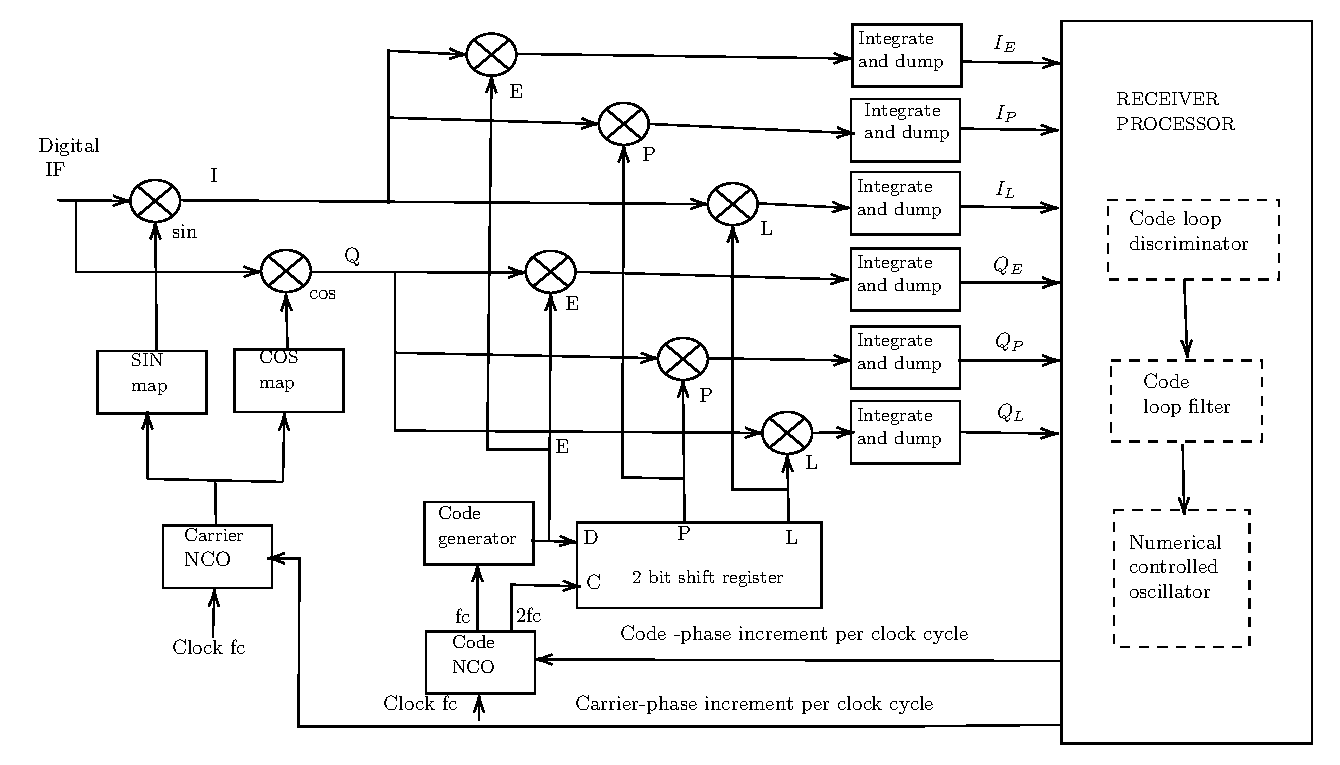
\includegraphics[scale=0.5]{figs/block3}
\end{figure}
%\end{normalsize}
%\begin{Large}
\begin{center}
Figure3 : Generic digital receiver channel
\end{center}
\begin{align}
\text{PLL Discriminator} =ATAN2(I_P,Q_P) = \tan^{-1}\brak{\frac{I_P}{Q_P}}
\end{align}
compares the phase error outputs of these PLL discriminators assuming no noise in the I and Q signals. Note that the ATAN2 discriminator is the only one that remains linear over the full input error range of $\pm180^{\circ}$. However, in the presence of noise, both of the discriminator outputs are linear only near the $0^{\circ}$ region. These PLL discriminators will achieve the 6-dB improvement in signal tracking threshold (by comparison with the Costas discriminators described next) for the dataless carrier because they track the full four quadrant range of the input signal.\\
\textbf{Frequency locked loop}\\
PLLs replicate the exact phase and frequency of the incoming SV (converted to IF) to perform the carrier wipeoff function. FLLs perform the carrier wipeoff process by replicating the approximate frequency, and they typically permit the phase to rotate with respect to the incoming carrier signal.
\begin{align}
\text{FLL Discriminator} =\frac{ATAN2(dot,cross)}{t2-t1}
\end{align}
ATAN2(dot, cross)FLL discriminators are equal to half the predetection bandwidths. The (cross)$\times$ sign(dot) FLL discriminator frequency pull-in ranges are only one-fourth of the predetection bandwidths. Also note that the (cross) $\times$ sign(dot) and the cross FLL discriminator outputs, whose outputs are sine functions divided by the sample time interval $(t_2 -t _1)$ in seconds, are also divided by 4 to more accurately approximate the true input frequency error. The ATAN2 (x, y) function returns the answer in radians, is converted to degrees, divided by the sample time interval $(t_2 - t_1)$in seconds,
and is also divided by 360 to produce at its output a true representation of the input
frequency error within its pull-in range
\subsection{Code tracking loop:}
\textbf{Delay locked loop}
Post the carrier signal synchronization, received CA code samples is synchronized by aligning with replicated CA code samples by shifting right or left. To determine the direction of shift, the I and Q outputs are multiplied with prompt code (PRN code which is phase aligned), early code (prompt PRN code shifted by some samples to the right) and late code (prompt PRN code shifted by some samples to the left) resulting in corresponding to I and Q channel respectively.IRNSS receiver delay lock loop (DLL) discriminators and their characteristics.

 \begin{align}
 E=\sqrt[]{I_{ES}^2+Q_{ES}^2}
 \end{align}
 \begin{align}
 L=\sqrt[]{I_{LS}^2+Q_{LS}^2}
 \end{align}
\begin{align}
\text{DLL Discriminator} (\epsilon)=\frac{1}{2}\frac{E-L}{E+L}
\end{align}
Noncoherent early minus late envelope normalized by $E + L$ to remove amplitude sensitivity High computational load.For  1-chip $E - L$ correlator spacing, produces true tracking error within $\pm 0.5$  chip of input error (in the absence of noise).
Becomes unstable (divide by zero) at $\pm 1.5$ -chip input error, but this is well beyond code tracking threshold in the presence of noise.
%\end{Large}\\
\subsection{Loop filter characteristics}
\begin{table}[h]
\centering
	\caption{\Large{Loop order filters }}
	%%%%%%%%%%%%%%%%%%%%%%%%%%%%%%%%%%%%%%%%%%%%%%%%%%%%%%%%%%%%%%%%%%%%%%
%%                                                                  %%
%%  This is the header of a LaTeX2e file exported from Gnumeric.    %%
%%                                                                  %%
%%  This file can be compiled as it stands or included in another   %%
%%  LaTeX document. The table is based on the longtable package so  %%
%%  the longtable options (headers, footers...) can be set in the   %%
%%  preamble section below (see PRAMBLE).                           %%
%%                                                                  %%
%%  To include the file in another, the following two lines must be %%
%%  in the including file:                                          %%
%%        \def\inputGnumericTable{}                                 %%
%%  at the beginning of the file and:                               %%
%%        \input{name-of-this-file.tex}                             %%
%%  where the table is to be placed. Note also that the including   %%
%%  file must use the following packages for the table to be        %%
%%  rendered correctly:                                             %%
%%    \usepackage[latin1]{inputenc}                                 %%
%%    \usepackage{color}                                            %%
%%    \usepackage{array}                                            %%
%%    \usepackage{longtable}                                        %%
%%    \usepackage{calc}                                             %%
%%    \usepackage{multirow}                                         %%
%%    \usepackage{hhline}                                           %%
%%    \usepackage{ifthen}                                           %%
%%  optionally (for landscape tables embedded in another document): %%
%%    \usepackage{lscape}                                           %%
%%                                                                  %%
%%%%%%%%%%%%%%%%%%%%%%%%%%%%%%%%%%%%%%%%%%%%%%%%%%%%%%%%%%%%%%%%%%%%%%



%%  This section checks if we are begin input into another file or  %%
%%  the file will be compiled alone. First use a macro taken from   %%
%%  the TeXbook ex 7.7 (suggestion of Han-Wen Nienhuys).            %%
\def\ifundefined#1{\expandafter\ifx\csname#1\endcsname\relax}


%%  Check for the \def token for inputed files. If it is not        %%
%%  defined, the file will be processed as a standalone and the     %%
%%  preamble will be used.                                          %%
\ifundefined{inputGnumericTable}

%%  We must be able to close or not the document at the end.        %%
	\def\gnumericTableEnd{\end{document}}


%%%%%%%%%%%%%%%%%%%%%%%%%%%%%%%%%%%%%%%%%%%%%%%%%%%%%%%%%%%%%%%%%%%%%%
%%                                                                  %%
%%  This is the PREAMBLE. Change these values to get the right      %%
%%  paper size and other niceties.                                  %%
%%                                                                  %%
%%%%%%%%%%%%%%%%%%%%%%%%%%%%%%%%%%%%%%%%%%%%%%%%%%%%%%%%%%%%%%%%%%%%%%

	\documentclass[12pt%
			  %,landscape%
                    ]{report}
       \usepackage[latin1]{inputenc}
       \usepackage{fullpage}
       \usepackage{color}
       \usepackage{array}
       \usepackage{longtable}
       \usepackage{calc}
       \usepackage{multirow}
       \usepackage{hhline}
       \usepackage{ifthen}

	\begin{document}


%%  End of the preamble for the standalone. The next section is for %%
%%  documents which are included into other LaTeX2e files.          %%
\else

%%  We are not a stand alone document. For a regular table, we will %%
%%  have no preamble and only define the closing to mean nothing.   %%
    \def\gnumericTableEnd{}

%%  If we want landscape mode in an embedded document, comment out  %%
%%  the line above and uncomment the two below. The table will      %%
%%  begin on a new page and run in landscape mode.                  %%
%       \def\gnumericTableEnd{\end{landscape}}
%       \begin{landscape}


%%  End of the else clause for this file being \input.              %%
\fi

%%%%%%%%%%%%%%%%%%%%%%%%%%%%%%%%%%%%%%%%%%%%%%%%%%%%%%%%%%%%%%%%%%%%%%
%%                                                                  %%
%%  The rest is the gnumeric table, except for the closing          %%
%%  statement. Changes below will alter the table's appearance.     %%
%%                                                                  %%
%%%%%%%%%%%%%%%%%%%%%%%%%%%%%%%%%%%%%%%%%%%%%%%%%%%%%%%%%%%%%%%%%%%%%%

\providecommand{\gnumericmathit}[1]{#1} 
%%  Uncomment the next line if you would like your numbers to be in %%
%%  italics if they are italizised in the gnumeric table.           %%
%\renewcommand{\gnumericmathit}[1]{\mathit{#1}}
\providecommand{\gnumericPB}[1]%
{\let\gnumericTemp=\\#1\let\\=\gnumericTemp\hspace{0pt}}
 \ifundefined{gnumericTableWidthDefined}
        \newlength{\gnumericTableWidth}
        \newlength{\gnumericTableWidthComplete}
        \newlength{\gnumericMultiRowLength}
        \global\def\gnumericTableWidthDefined{}
 \fi
%% The following setting protects this code from babel shorthands.  %%
 \ifthenelse{\isundefined{\languageshorthands}}{}{\languageshorthands{english}}
%%  The default table format retains the relative column widths of  %%
%%  gnumeric. They can easily be changed to c, r or l. In that case %%
%%  you may want to comment out the next line and uncomment the one %%
%%  thereafter                                                      %%
\providecommand\gnumbox{\makebox[0pt]}
%%\providecommand\gnumbox[1][]{\makebox}

%% to adjust positions in multirow situations                       %%
\setlength{\bigstrutjot}{\jot}
\setlength{\extrarowheight}{\doublerulesep}

%%  The \setlongtables command keeps column widths the same across  %%
%%  pages. Simply comment out next line for varying column widths.  %%
\setlongtables

\setlength\gnumericTableWidth{%
	70pt+%
	100pt+%
	80pt+%
0pt}
\def\gumericNumCols{3}
\setlength\gnumericTableWidthComplete{\gnumericTableWidth+%
         \tabcolsep*\gumericNumCols*2+\arrayrulewidth*\gumericNumCols}
\ifthenelse{\lengthtest{\gnumericTableWidthComplete > \linewidth}}%
         {\def\gnumericScale{\ratio{\linewidth-%
                        \tabcolsep*\gumericNumCols*2-%
                        \arrayrulewidth*\gumericNumCols}%
{\gnumericTableWidth}}}%
{\def\gnumericScale{1}}

%%%%%%%%%%%%%%%%%%%%%%%%%%%%%%%%%%%%%%%%%%%%%%%%%%%%%%%%%%%%%%%%%%%%%%
%%                                                                  %%
%% The following are the widths of the various columns. We are      %%
%% defining them here because then they are easier to change.       %%
%% Depending on the cell formats we may use them more than once.    %%
%%                                                                  %%
%%%%%%%%%%%%%%%%%%%%%%%%%%%%%%%%%%%%%%%%%%%%%%%%%%%%%%%%%%%%%%%%%%%%%%

\ifthenelse{\isundefined{\gnumericColA}}{\newlength{\gnumericColA}}{}\settowidth{\gnumericColA}{\begin{tabular}{@{}p{70pt*\gnumericScale}@{}}x\end{tabular}}
\ifthenelse{\isundefined{\gnumericColB}}{\newlength{\gnumericColB}}{}\settowidth{\gnumericColB}{\begin{tabular}{@{}p{100pt*\gnumericScale}@{}}x\end{tabular}}
\ifthenelse{\isundefined{\gnumericColC}}{\newlength{\gnumericColC}}{}\settowidth{\gnumericColC}{\begin{tabular}{@{}p{80pt*\gnumericScale}@{}}x\end{tabular}}

\begin{longtable}[c]{%
	b{\gnumericColA}%
	b{\gnumericColB}%
	b{\gnumericColC}%
	}

%%%%%%%%%%%%%%%%%%%%%%%%%%%%%%%%%%%%%%%%%%%%%%%%%%%%%%%%%%%%%%%%%%%%%%
%%  The longtable options. (Caption, headers... see Goosens, p.124) %%
%	\caption{The Table Caption.}             \\	%
% \hline	% Across the top of the table.
%%  The rest of these options are table rows which are placed on    %%
%%  the first, last or every page. Use \multicolumn if you want.    %%

%%  Header for the first page.                                      %%
%	\multicolumn{3}{c}{The First Header} \\ \hline 
%	\multicolumn{1}{c}{colTag}	%Column 1
%	&\multicolumn{1}{c}{colTag}	%Column 2
%	&\multicolumn{1}{c}{colTag}	\\ \hline %Last column
%	\endfirsthead

%%  The running header definition.                                  %%
%	\hline
%	\multicolumn{3}{l}{\ldots\small\slshape continued} \\ \hline
%	\multicolumn{1}{c}{colTag}	%Column 1
%	&\multicolumn{1}{c}{colTag}	%Column 2
%	&\multicolumn{1}{c}{colTag}	\\ \hline %Last column
%	\endhead

%%  The running footer definition.                                  %%
%	\hline
%	\multicolumn{3}{r}{\small\slshape continued\ldots} \\
%	\endfoot

%%  The ending footer definition.                                   %%
%	\multicolumn{3}{c}{That's all folks} \\ \hline 
%	\endlastfoot
%%%%%%%%%%%%%%%%%%%%%%%%%%%%%%%%%%%%%%%%%%%%%%%%%%%%%%%%%%%%%%%%%%%%%%

\hhline{|-|-|-}
	 \multicolumn{1}{|p{\gnumericColA}|}%
	{\gnumericPB{\raggedright}\gnumbox[l]{\textbf{Loop Order}}}
	&\multicolumn{1}{p{\gnumericColB}|}%
	{\gnumericPB{\raggedright}\gnumbox[l]{\textbf{Noise Bandwidth}}}
	&\multicolumn{1}{p{\gnumericColC}|}%
	{\gnumericPB{\raggedright}\gnumbox[l]{\textbf{Typical Filter  }}}
\\
%\hhline{|---|}
	 \multicolumn{1}{|p{\gnumericColA}|}%
	{\gnumericPB{\raggedleft}\gnumbox[r]{}}
	&\multicolumn{1}{p{\gnumericColB}|}%
	{\gnumericPB{\raggedright}\gnumbox[l]{\textbf{$ B_n$ (Hz)}}}
	&\multicolumn{1}{p{\gnumericColC}|}%
	{\gnumericPB{\raggedright}\gnumbox[l]{\textbf{ Values }}}
	%{\gnumericPB{\raggedright}\gnumbox[l]{}}\\
	\\
\hhline{|---|}
	 \multicolumn{1}{|p{\gnumericColA}|}%
	{\gnumericPB{\raggedleft}\gnumbox[r]{First}}
	&\multicolumn{1}{p{\gnumericColB}|}%
	{\gnumericPB{\raggedright}\gnumbox[l]{\hspace{0.5cm}$\frac{\omega_o}{4}$}}
	&\multicolumn{1}{p{\gnumericColC}|}%
	{\gnumericPB{\raggedright}\gnumbox[l]{\hspace{0.5cm}$\omega_o $ }}
	%{\gnumericPB{\raggedright}\gnumbox[l]{}}\\
	\\
%\hhline{|---|}
	 \multicolumn{1}{|p{\gnumericColA}|}%
	{\gnumericPB{\raggedleft}\gnumbox[r]{}}
	&\multicolumn{1}{p{\gnumericColB}|}%
	{\gnumericPB{\raggedright}\gnumbox[l]{}}
	&\multicolumn{1}{p{\gnumericColC}|}%
	{\gnumericPB{\raggedright}\gnumbox[l]{ $B_n=0.25\omega_o$}}
\\
\hhline{|---|}
\multicolumn{1}{|p{\gnumericColA}|}%
	{\gnumericPB{\raggedleft}\gnumbox[r]{}}
	&\multicolumn{1}{p{\gnumericColB}|}%
	{\gnumericPB{\raggedright}\gnumbox[l]{}}
	&\multicolumn{1}{p{\gnumericColC}|}%
	{\gnumericPB{\raggedright}\gnumbox[l]{ $\omega_o^2$}}
	 
\\
%\hhline{|---|}
	\multicolumn{1}{|p{\gnumericColA}|}%
	{\gnumericPB{\raggedleft}\gnumbox[r]{Second}}
	&\multicolumn{1}{p{\gnumericColB}|}%
	{\gnumericPB{\raggedright}\gnumbox[l]{$\frac{\omega(1+a_2^2)}{4a_2}$}}
	&\multicolumn{1}{p{\gnumericColC}|}%
	{\gnumericPB{\raggedright}\gnumbox[l]{$a_2\omega_o=1.414\omega_o$}}
\\
%\hhline{|-|-|-|}
\multicolumn{1}{|p{\gnumericColA}|}%
	{\gnumericPB{\raggedleft}\gnumbox[r]{}}
	&\multicolumn{1}{p{\gnumericColB}|}%
	{\gnumericPB{\raggedright}\gnumbox[l]{}}
	&\multicolumn{1}{p{\gnumericColC}|}%
	{\gnumericPB{\raggedright}\gnumbox[l]{ $B_n=0.53\omega_o$}}
	
	\\
\hhline{|-|-|-|}
 \multicolumn{1}{|p{\gnumericColA}|}%
	{\gnumericPB{\raggedleft}\gnumbox[r]{}}
	&\multicolumn{1}{p{\gnumericColB}|}%
	{\gnumericPB{\raggedright}\gnumbox[l]{}}
	&\multicolumn{1}{p{\gnumericColC}|}%
	{\gnumericPB{\raggedright}\gnumbox[l]{$\omega_o^3$ }}
		\\
%\hhline{|-|-|-|}
 \multicolumn{1}{|p{\gnumericColA}|}%
	{\gnumericPB{\raggedleft}\gnumbox[r]{Third}}
	&\multicolumn{1}{p{\gnumericColB}|}%
	{\gnumericPB{\raggedright}\gnumbox[l]{$\frac{\omega(a_3b_3^2+a_3^2-b_3)}{4(a_3b_3-1)}$}}
	&\multicolumn{1}{p{\gnumericColC}|}%
	{\gnumericPB{\raggedright}\gnumbox[l]{$ a_3\omega_o^2=1.1\omega_o^2$}}
	\\
%\hhline{|-|-|-|}
 \multicolumn{1}{|p{\gnumericColA}|}%
	{\gnumericPB{\raggedleft}\gnumbox[r]{}}
	&\multicolumn{1}{p{\gnumericColB}|}%
	{\gnumericPB{\raggedright}\gnumbox[l]{}}
	&\multicolumn{1}{p{\gnumericColC}|}%
	{\gnumericPB{\raggedright}\gnumbox[l]{$b_3\omega_o=2.4\omega_o$}}
	\\
%\hhline{|-|-|-|}
 \multicolumn{1}{|p{\gnumericColA}|}%
	{\gnumericPB{\raggedleft}\gnumbox[r]{}}
	&\multicolumn{1}{p{\gnumericColB}|}%
	{\gnumericPB{\raggedright}\gnumbox[l]{}}
	&\multicolumn{1}{p{\gnumericColC}|}%
	{\gnumericPB{\raggedright}\gnumbox[l]{ $B_n=0.7845\omega_o$}}
		\\
\hhline{|-|-|-|}
 
\end{longtable}

\ifthenelse{\isundefined{\languageshorthands}}{}{\languageshorthands{\languagename}}
\gnumericTableEnd

\end{table}

The values for the second-order coefficient $a_2$ and third-order coefficients $a_3$ and $b_3$ can be determined from Table 3. These coefficients are the same for FLL, PLL, or DLL applications if the loop
order and the noise bandwidth,$B_n$ , are the same.Note that the FLL coefficient insertion point into the filter is one integrator back from the PLL and DLL insertion points.This is because the FLL error is in units of hertz (change in range per unit of time).\\
The tracking results are generated using the below code\\
\textbf{Code}
\begin{lstlisting}
code/e2e_sim/main_ipynb
\end{lstlisting}
\textbf{Result}
\begin{lstlisting}
Tracking result for PRN ID:5
Transmitted Bits:
 [0. 1. 0. 1. 0. 0. 0. 1. 0. 1. 1. 0. 0. 0. 1. 1. 1. 0. 0. 1. 1. 1. 1. 0.1. 0. 1. 1. 0. 1. 0. 0. 1. 0. 0. 0. 1. 0. 1. 1. 1. 0. 1. 1. 0. 0. 1. 0. 0. 0.]
Received bits:
 [1. 1. 0. 1. 0. 1. 1. 1. 0. 1. 0. 0. 1. 1. 1. 0. 0. 0. 1. 1. 0. 0. 0. 0.1. 0. 1. 0. 0. 1. 0. 1. 1. 0. 1. 1. 1. 0. 1. 0. 0. 0. 1. 0. 0. 1. 1. 0.1. 1.]
Received bits inverted:
 [0. 0. 1. 0. 1. 0. 0. 0. 1. 0. 1. 1. 0. 0. 0. 1. 1. 1. 0. 0. 1. 1. 1. 1.0. 1. 0. 1. 1. 0. 1. 0. 0. 1. 0. 0. 0. 1. 0. 1. 1. 1. 0. 1. 1. 0. 0. 1. 0. 0.]
\end{lstlisting}

\begin{figure}[H]
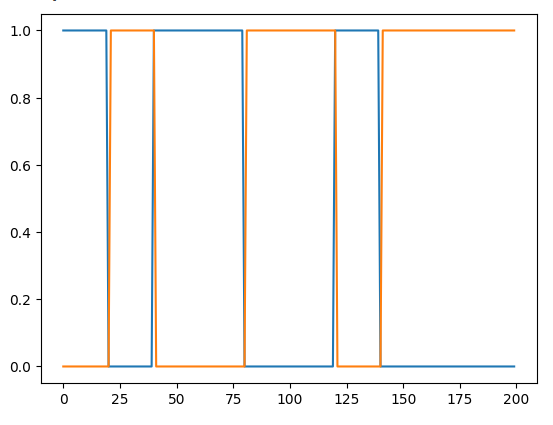
\includegraphics[width=0.5\columnwidth]{figs/tracking_plot.png}
\caption{tracking result plot}
\end{figure}

The functions for acquisition and tracking are present in the below code
\begin{lstlisting}
codes/demodulation/demodulation.py
\end{lstlisting}


%\end{Large}

%\end{enumerate}
%\end{document}
